\chapter{Theoretical Background}

\section{Convolutional Neural Networks (CNNs)}

\subsection{Introduction to CNNs}

Convolutional Neural Networks (CNNs) are a class of deep learning models that have gained widespread popularity due to their ability to effectively analyze visual data. Originally inspired by the organization of the animal visual cortex, CNNs are a perfect tool for image recognition tasks.

A distinctive feature of CNNs is their ability to capture local dependencies in images using convolutional layers. These layers apply trainable filters (or kernels) over the input image to detect various features such as edges, textures, and patterns. As the network deepens, it gradually captures more complex and abstract features, which allows for highly accurate image classification.

\subsection{Architecture of CNNs}

A typical CNN architecture consists of several key components: an input layer, convolutional layers, pooling layers, and fully connected layers. Each component plays a specific role in processing the input data and contributing to the overall functionality of the network.

\begin{figure}[h]
    \centering
    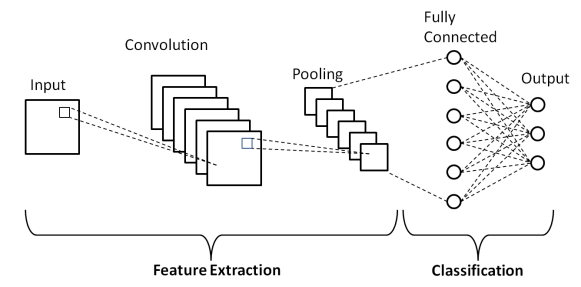
\includegraphics[width=0.7\textwidth]{img/cnn-architecture.png}
    \caption{Illustration of a CNN architecture. Source: \href{https://www.researchgate.net/publication/336805909_A_High-Accuracy_Model_Average_Ensemble_of_Convolutional_Neural_Networks_for_Classification_of_Cloud_Image_Patches_on_Small_Datasets}{ResearchGate article.}}\label{fig:cnn-architecture}
\end{figure}

\subsubsection{Convolutional Layers}

Convolutional layers are the main building block of a CNN architecture. They apply a set of filters over the input image, where each filter slides (or convolves) across the image to produce a feature map. This operation helps the network learn spatial hierarchies of features, where earlier layers might detect simple edges or textures, and deeper layers capture more complex structures like shapes or even entire objects.

The mathematical operation behind convolution involves multiplying each filter's weights by the corresponding pixel values in the input image and summing the results. This process is repeated as the filter moves across the image, resulting in a feature map that highlights the presence of the feature detected by the filter.

Mathematically, the convolution operation for a single filter can be expressed as:

\[
\text{FeatureMap}(i,j) = \sum_{m,n} I_{i-m,j-n} W_{m,n} + b
\]

where \(W\) represents the filter weights, \(I\) represents the input image pixel values, and \(b\) is the bias term.

\subsubsection{Activation Functions}

After convolution, the output feature map is passed through a non-linear activation function, typically the Rectified Linear Unit (ReLU). The ReLU activation function is defined as:

\[
ReLU(x) = \max(0, x)
\]

ReLU introduces non-linearity into the model, which is needed in order to learn more complex patterns in the data. Other activation functions, for example hyperbolic tangent (tanh), can also be used, but ReLU is preferred in most CNN architectures due to its simplicity and effectiveness in avoiding the vanishing gradient problem.

\subsubsection{Pooling Layers}

Pooling layers, often placed between consecutive convolutional layers, are used to reduce the dimensions of the feature maps. This operation reduces the network's computational complexity and makes the learned features more invariant to small translations of the input image.

The most common pooling operation is max pooling, which selects the maximum value from each region of the feature map. The formula for max pooling over a 2x2 region is:

\[
\text{MaxPool}(i,j) = \max \{ I_{2i,2j}, I_{2i,2j+1}, I_{2i+1,2j}, I_{2i+1,2j+1} \}
\]

Another popular type of pooling operation is average pooling, which computes the region's average value instead of the maximum.

Overall, pooling layers gradually reduce the spatial size of the image representation, making the network more efficient while retaining the most important features. 

\subsubsection{Fully Connected Layers}

After several convolutional and pooling layers, the resulting feature maps are flattened into a one-dimensional vector to be processed by one or more fully connected layers. These layers function like a standard neural network, where each neuron is linked to every neuron in the next layer. Finally, the last fully connected layer, called the output layer, performs the final classification.

The CNN's output layer typically uses a softmax activation function for multi-class classification tasks. The softmax function converts the output scores into probabilities, allowing the network to assign a class label to the input image.

\subsection{Conclusion}

CNNs have been successfully used to solve various image classification tasks, including object detection, face recognition, and medical image analysis. In the context of museum applications, CNNs are used to classify and recognize various types of exhibits, ranging from paintings and sculptures to historical artifacts. By fine-tuning pre-trained CNN models on museum-specific datasets, it is possible to achieve high accuracy in identifying exhibits, thereby enhancing the visitor experience.

\section{MobileNet}\label{section:mobilenet}

MobileNet is a class of efficient convolutional neural networks specifically designed for mobile and embedded vision applications. Introduced by Howard et al. \cite{howard_mobilenet}, MobileNet addresses the need for high-performance neural networks that can work efficiently on devices with limited resources (e.g., smartphones).

\subsection{Architecture of MobileNet}

The core innovation of MobileNet is the use of depthwise separable convolutions, which break down the standard convolution operation into two simpler steps: depthwise convolution (applying a single filter per input channel) and pointwise convolution (combining the output channels). This approach significantly reduces the number of calculations (23x fewer multiplications for an 8x8x3 image) and model size, making MobileNet fast and lightweight.

\begin{figure}[h]
    \centering
    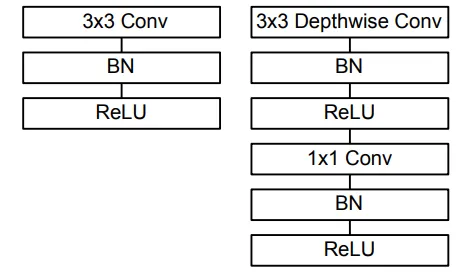
\includegraphics[width=0.7\textwidth]{img/mobilenet.png}
    \caption{Left: Standard Convolutional layer, Right: Depthwise Separable Convolutional layers in MobileNet. Source: image from the original paper.}
    \label{fig:mobilenet}
\end{figure}

\subsection{MobileNet Versions}

There are three versions of the MobileNet architecture, each improving upon the last in terms of efficiency and accuracy:

\textbf{MobileNetV1} was the first iteration, known for being ten times faster and smaller than the VGG16 architecture, making it a popular choice for mobile applications due to its significant reduction in computational resources \cite{pandrii_mobilenet}.

\textbf{MobileNetV2} introduced inverted residual blocks with linear bottlenecks, which enhanced the model's ability to learn more efficient representations. This version is approximately 30\% smaller and 0.3 times faster than MobileNetV1 while being 1\% more accurate \cite{pandrii_mobilenet}.

\textbf{MobileNetV3} builds upon the improvements of V2 by incorporating advances such as Neural Architecture Search (NAS) and Squeeze-and-Excitation (SE) modules. MobileNetV3 is twice as fast and 30\% smaller than V2 but with a slight trade-off in accuracy, being 3\% less accurate than MobileNetV2 \cite{pandrii_mobilenet}.

\textbf{Note on Model Choice:} Despite the improvements in MobileNetV3, MobileNetV2 was chosen for this thesis due to its optimal balance between accuracy and efficiency. While V3 offers better speed and smaller size, the slight reduction in accuracy was not suitable for the high accuracy requirements of this project.

\subsection{Conclusion}

Thanks to its efficient design, MobileNet offers a well-balanced architecture ideal for real-time applications on mobile devices. In this thesis, MobileNet's lightweight structure is crucial for effectively and accurately classifying museum exhibits, providing visitors with enhanced learning experiences while maintaining optimal performance on mobile hardware.

\section{Transfer Learning}\label{section:transfer_learning}

\subsection{Introduction to Transfer Learning}

Transfer learning is a machine learning technique of using knowledge gained during the execution of one task to improve the performance of another related task. Instead of building and training a new model from scratch, scientists and engineers can use pre-trained models as a starting point, reducing the need for large amounts of data and computational resources.

In traditional machine learning, models are usually trained from scratch using a large dataset for a specific task. This process involves learning feature representations from the raw data, which can be time-consuming and computationally intensive. However, the early layers of neural networks often learn general features like edges and textures that are useful across tasks, so transfer learning takes advantage of these general features by reusing the early layers of a pre-trained model and fine-tuning the later layers on the target task. The most common approach to transfer learning involves:

1. \textbf{Pre-training:} A model is first trained on a large source dataset with extensive labeled examples (e.g., ImageNet). During this phase, the model learns to extract general features from the input data.

2. \textbf{Fine-tuning:} The pre-trained model is then adapted to the target task by continuing training on a smaller, task-specific dataset. This process fine-tunes the model's weights to better fit the characteristics of the target data while retaining the knowledge acquired during pre-training.

\subsection{Transfer Learning in CNNs}

Transfer learning is widely used in the context of CNNs, especially for image classification tasks. During transfer learning, the early layers of a pre-trained CNN are often frozen (i.e., their weights are kept constant), and only the deeper layers are fine-tuned. This approach keeps the general feature extraction capabilities of the early layers, which are often relevant across different tasks, while adapting the model to the specific characteristics of the target data.

\subsection{Transfer Learning in Museum Exhibit Classification}

In the context of museum exhibit classification, transfer learning is beneficial due to the limited availability of labeled data for training. Museum exhibits vary widely in style, material, and content, making it difficult to compile a comprehensive dataset. By using a pre-trained CNN model like MobileNet, which has been trained on a large, diverse dataset such as ImageNet, it is possible to effectively classify museum exhibits with a smaller, domain-specific dataset.

\subsection{Conclusion}

Transfer learning enables the reuse of pre-trained models to solve new tasks with limited data and resources. In this thesis, transfer learning is crucial for developing an efficient and accurate model for museum exhibit classification, ensuring high-quality performance on mobile devices.